\begin{frame}{Optimization - Setup}
    \begin{columns}[c,onlytextwidth]
    \begin{column}{0.6\textwidth}
    BRs from minimization through
    \texttt{MINUIT}/{\color{llblue}\href{https://github.com/scikit-hep/iminuit}{iminuit}}.
    \begin{itemize}
        \item \texttt{MC2}:
              % Events that are (statistically) independent from \texttt{MC1}.
              Will be replaced by the detector data.
        \item $\vec{S} = M \cdot \vec{B} = \vec{f}(\vec{B})$, with
        \begin{itemize}
            \item $\vec{S}$: The signal counts per category ($S = data - bkg$). \texttt{MC2}.
            \item $M$: The matrix built from simulated events, as outlined above. \texttt{MC1}.
            \item $\vec{B}$: The target.
                  Use e.g. the Standard Model BRs as fit starting values.
        \end{itemize}
    %    \item The cost function: Currently Least Squares.
    %     \begin{itemize}
    %        \item $S$: The 1$\sigma$ binomial uncertainties on $S$ are the
    %             (only) place where the integrated luminosity effects the analysis.
    %        \item $M$:  Least Squares is not ideal: We discard known information
    %         (the total number of events in the sample).
    %     \end{itemize}
        \item The cost function: Multinomial log-likelihood.
        \begin{itemize}
            \item $- \tn{ln}\mathcal{L} = - N_{\tn{data}} \sum_i S_i \tn{ln}\left(\sum_j M_{ij}B_j\right)$.
            \item $B_{H \to ZZ^*} = 1 - \sum_{i \neq H \to ZZ^*} B_i$.
            % \item Each BR constrained to $\left[0, 1\right]$.
        \end{itemize}
    \end{itemize}
    \end{column}
    \begin{column}{0.4\textwidth}
    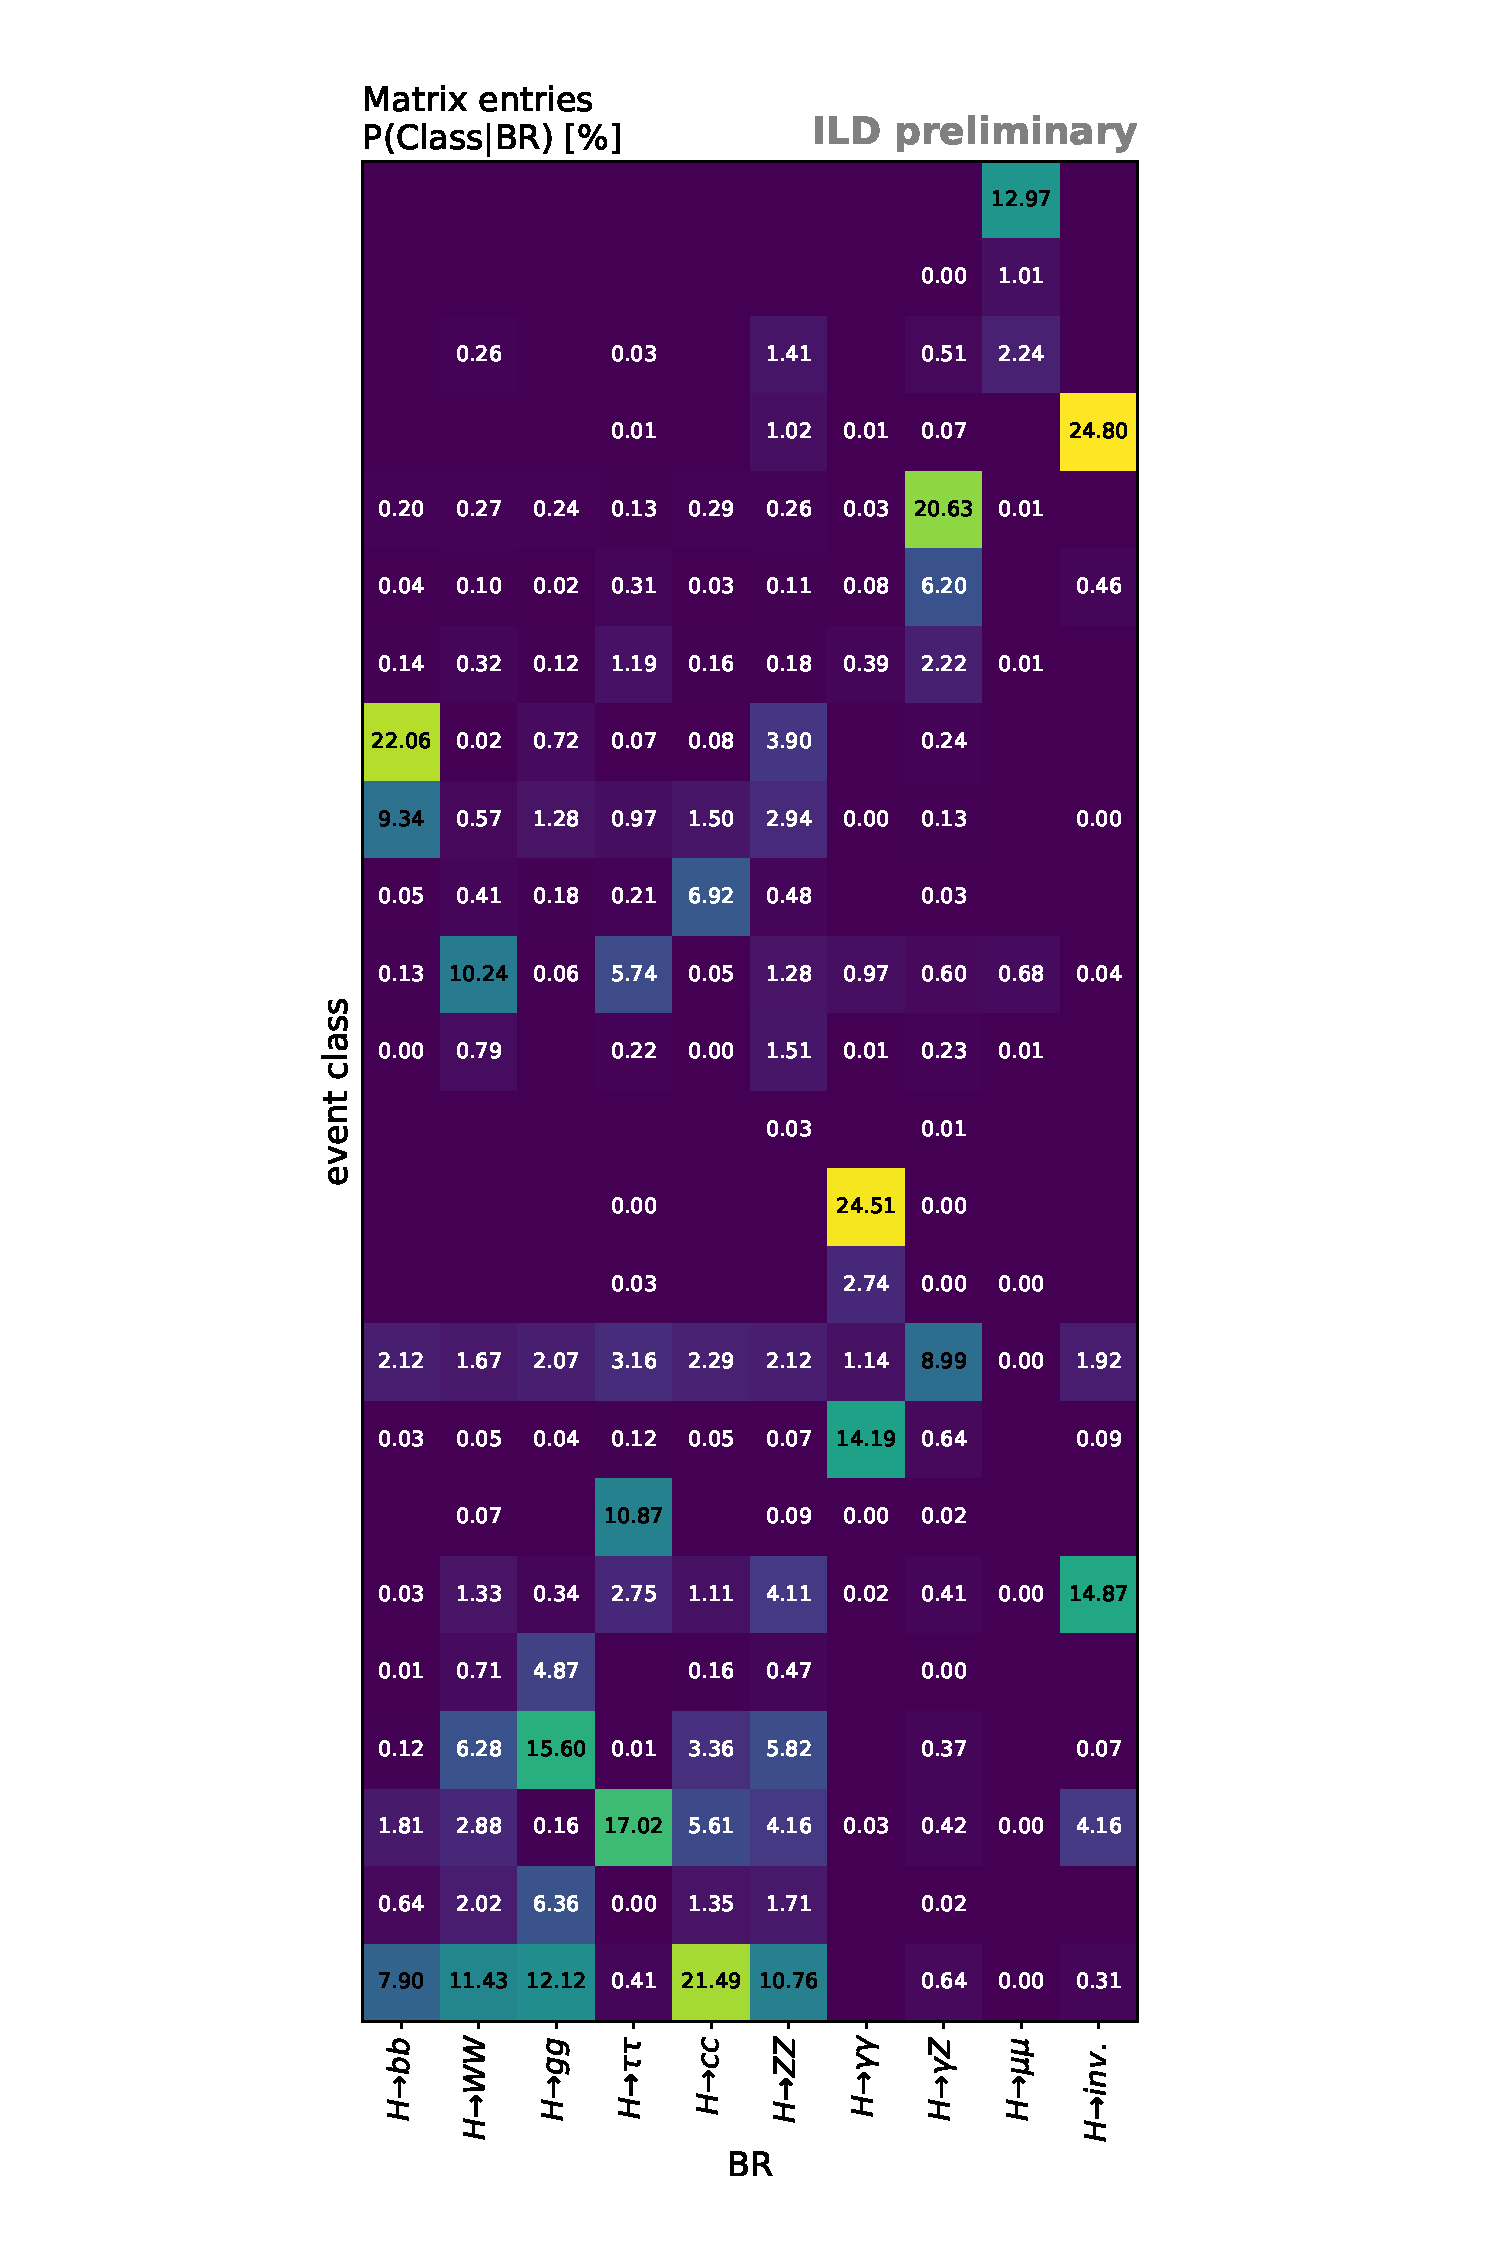
\includegraphics[height=0.85\textheight, width=0.95\textwidth, keepaspectratio]
        {probability_matrix}
    \end{column}
    \end{columns}
    \end{frame}
